\chapter{\label{a4-tf}Transfer Function Investigations}

\minitoc

\section{Introduction}

In the upgrade from \gls{target5} to \gls{targetc}, the ability to internally set the \gls{vped} to a known voltage was lost. The approach adopted to replace the Transfer Function generation was to input pulses of the correct shape into the module from an external pulse generator. However, this approach can only be done for one module at a time, outside the camera enclosure. As a result, we must rely on the Transfer Function data already taken for the generation of Transfer Functions for the \gls{target} modules currently installed in the \gls{chec-s} prototype. However, there are different options for how to approach the second step in the \gls{ac} Transfer Function generation (Chapter~\ref{ch5-calibration}). This appendix will explore the performance I obtained with different expressions of the Transfer Function.

\section{TF Generation Approaches}

\begin{figure}
	\centering
	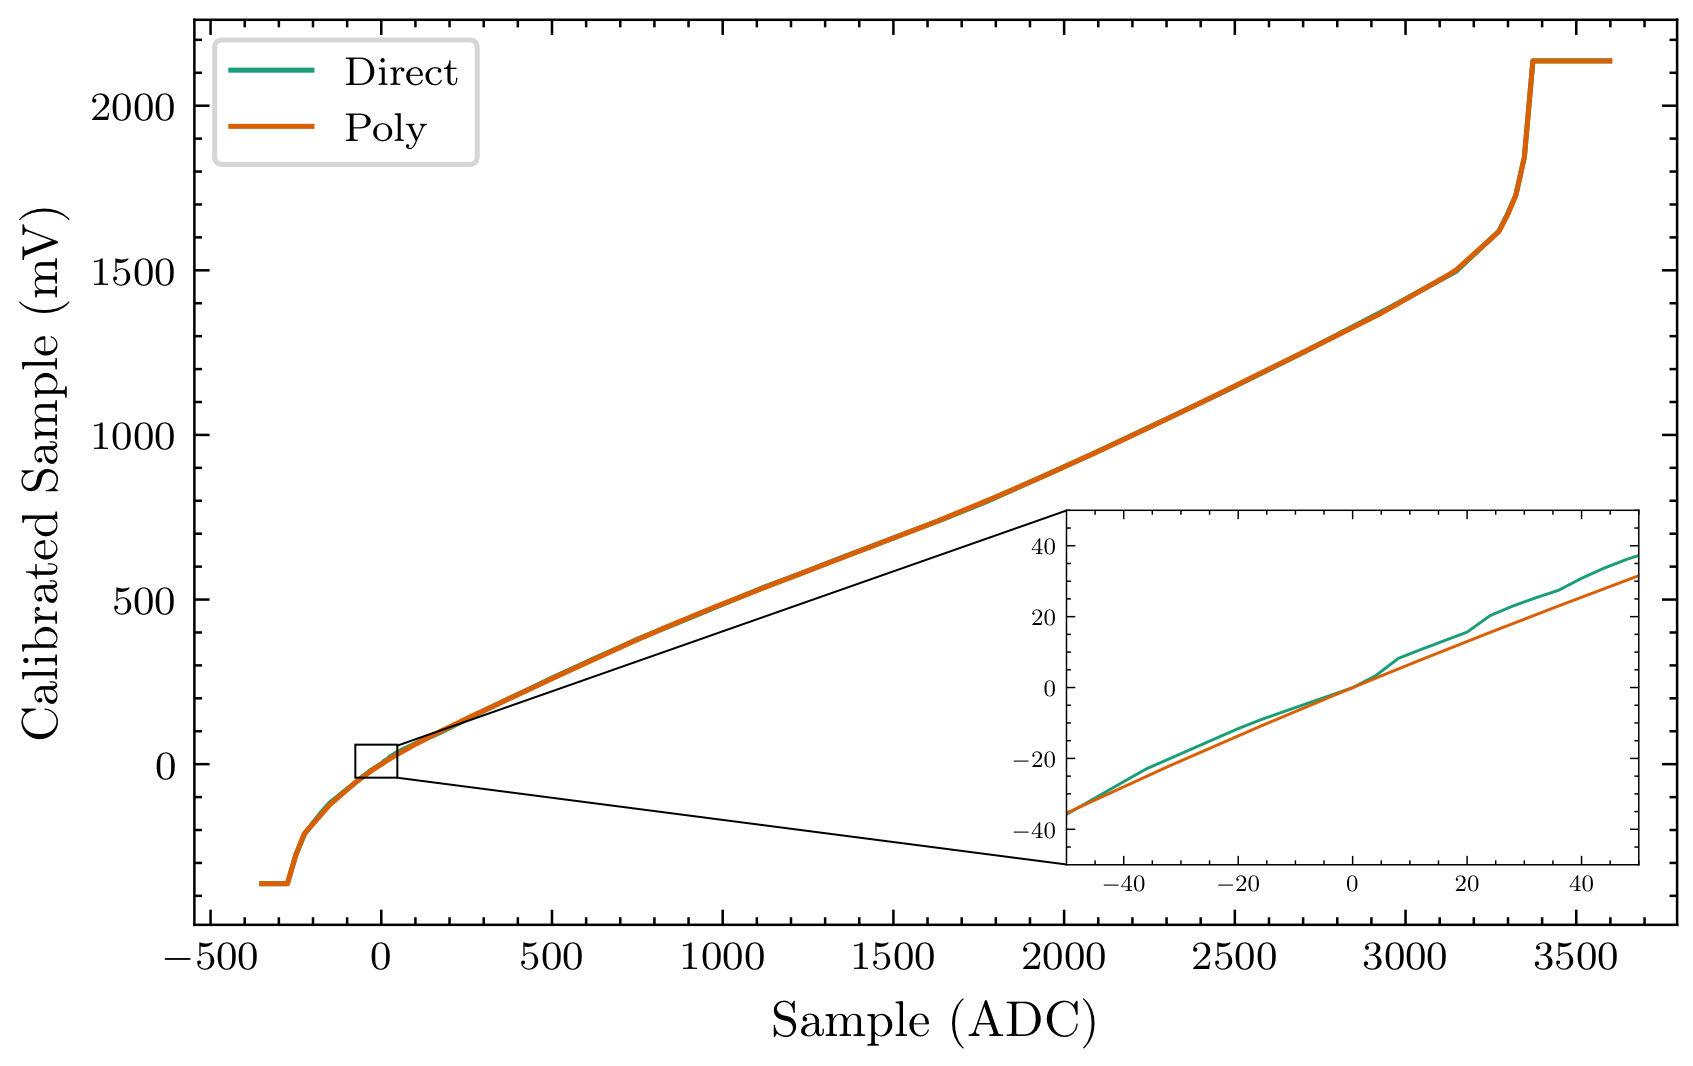
\includegraphics[width=\textwidth]{poly} 
	\caption[Comparison of the \textit{Poly} and \textit{Direct} Transfer Function lookup tables.]{Comparison of the \textit{Poly} and \textit{Direct} Transfer Function lookup tables, including a zoom at low amplitudes.} 
	\label{fig:poly}
\end{figure}

Four \gls{ac} Transfer Function generation approaches are considered:
\begin{enumerate}
\item \textit{Direct} - The values extracted from the waveforms are directly used, and a linear interpolation is performed to generate the lookup table.
\item \textit{PCHIP} - The low amplitude values are ignored as the waveform fit may not have performed reliably at that level. A Piecewise Cubic Hermite Interpolating Polynomial (PCHIP) is used to generate the lookup table as opposed to a linear interpolation, resulting in a smooth function.
\item \textit{Poly} - The Transfer Function of the \textit{Direct} approach is regressed with a high order polynomial. In this exercise a 14th order polynomial was used, however a much lower polynomial is sufficient if the saturated region is ignored. The difference between the \textit{Poly} and \textit{Direct} Transfer Function lookup tables for a single cell are shown in Figure~\ref{fig:poly}. The zoom in the figure shows the much smoother function for the \textit{Poly} approach.
\item \textit{None} - No Transfer Function calibration is applied. The pedestal subtraction calibration is still applied to the waveforms. Technically not a generation approach, but will give a benchmark to compare against.
\end{enumerate}

\section{Charge Resolution}

\begin{figure}
	\centering
	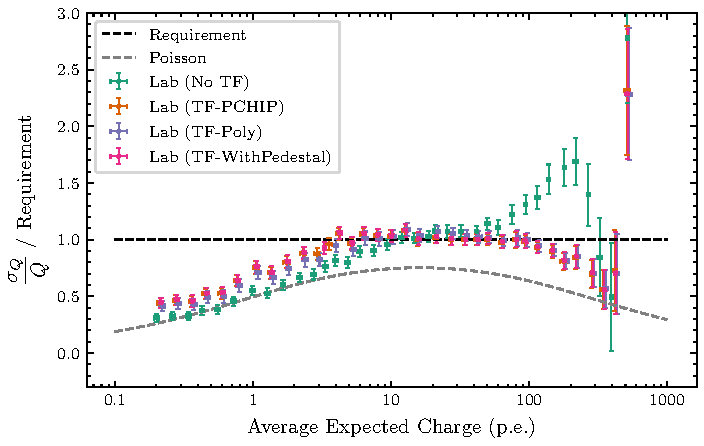
\includegraphics[width=\textwidth]{cr_6_tf_comparison} 
	\caption[Comparison of the \textit{Charge Resolution} resulting from each of the Transfer Function generation approaches.]{Comparison of the \textit{Charge Resolution} resulting from each of the Transfer Function generation approaches.} 
	\label{fig:cr_6_tf_comparison}
\end{figure}

The same dataset for the lab measurements shown in Chapter~\ref{ch7-performance} is used, but the different Transfer Function lookup tables are applied for the waveform calibration in each case. The filter-wheel calibration, flat-field calibration and charge extraction is also re-performed for each Transfer Function. Figure~\ref{fig:cr_6_tf_comparison} compares the \textit{Charge Resolution} result for each approach, allowing the following to be inferred:
\begin{itemize}
	\item The PCHIP interpolation results in only a minor improvement over the linear interpolation used for the \textit{Direct} approach.
	\item The use of a polynomial regression to express the Transfer appears to be the most successful Transfer Function approach.
	\item No significant difference between the generation approaches is observed above an average expected charge of \SI{10}{\pe}, suggesting the performance above that value is not dominated by the Transfer Function calibration.
	\item The \textit{Charge Resolution} in the absence of a Transfer Function calibration performs extremely well, approaching the poisson limit, for charges up to \SI{30}{\pe}. This result is significantly better than the results observed in all cases where a Transfer Function calibration was applied. This suggests the Transfer Function calibration, in its current form, is introducing an additional noise factor to the baseline.
	\item The \textit{Charge Resolution} does perform significantly worse above an expected charge of \SI{30}{\pe} when no Transfer Function calibration is applied to the waveforms.
\end{itemize}
An ideal Transfer Function calibration would result in the low amplitude performance currently observed in the absence of the calibration, while retaining its non-linearity correction at higher amplitudes to maintain the performance. A Transfer Function calibration that only corrects large amplitudes may be a more favourable approach, therefore avoiding additional noise at the low amplitude level.

\section{Sampling Cell versus Storage Cell}

\begin{figure}
	\centering
	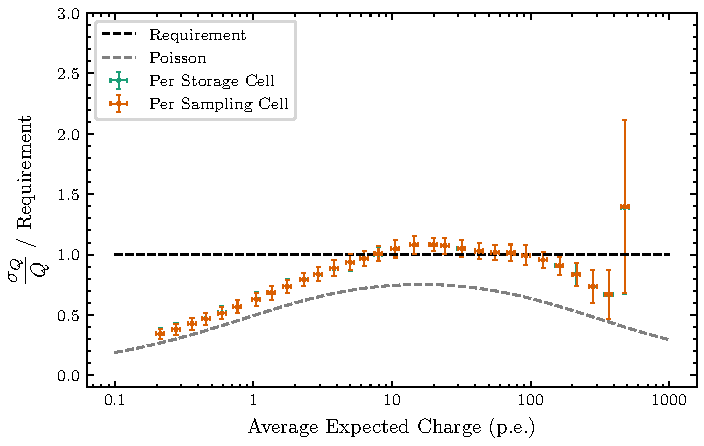
\includegraphics[width=\textwidth]{cr_6_tf_comparison_cells} 
	\caption[Comparison of the \textit{Charge Resolution} from the ``per sampling cell'' versus ``per storage cell''.]{Comparison of the \textit{Charge Resolution} resulting from a Transfer Function calibration in which each sampling cell has its own lookup table, versus one where each storage cell has a lookup table.} 
	\label{fig:cr_6_tf_comparison_cells}
\end{figure}

One further comparison approach performed for the Transfer Function calibration was between storing a lookup table per sampling cell or per storage cell. The former would result in 64 Transfer Functions per channel, the latter in 4,096 Transfer Functions per channel (for \gls{chec-s}). The \textit{Charge Resolution} results of this comparison are shown in Figure~\ref{fig:cr_6_tf_comparison_cells}. In both cases, the \textit{Poly} approach for generating the lookup table was used.

Despite investigations performed by other \gls{chec} members concluding that an improvement is found by considering a Transfer Function per storage cell, I observe no improvement in the \textit{Charge Resolution} results. This discrepancy between my conclusion and the conclusion obtained by others is likely due to the other more dominating contributions to the \textit{Charge Resolution}. Assuming a cell-level Transfer Function calibration is kept, this investigation should be repeated in future iterations of the \gls{chec} prototype, as the reduction in the other contributions may make the relative difference between ``per storage cell'' and ``per sampling cell'' more significant. If no significant distinction is found, the ``per sampling cell'' should be used due to the smaller number of lookup tables required.

\section{Conclusion}

It was concluded from these results that the best Transfer Function calibration currently available for \gls{chec} is provided by the \textit{Poly} generation approach, with a lookup table stored per storage cell. Therefore, this was the calibration approach used for this thesis.